This chapter will address the core experimental aspect of the assignment: the configuration of the load test and the procedure by which it is launched.
Subsequently, the final experimental outcomes will be presented.

\section{JMeter – load test configuration}

In the ``User Defined Variables'' module, the address of the computer running the RESTful API was entered.
All other components of the load test are contained in a ``Transaction controller'', which allows the system's throughput and expected response time to be measured, rather than the user's.
\begin{figure}[h]
	\centering
	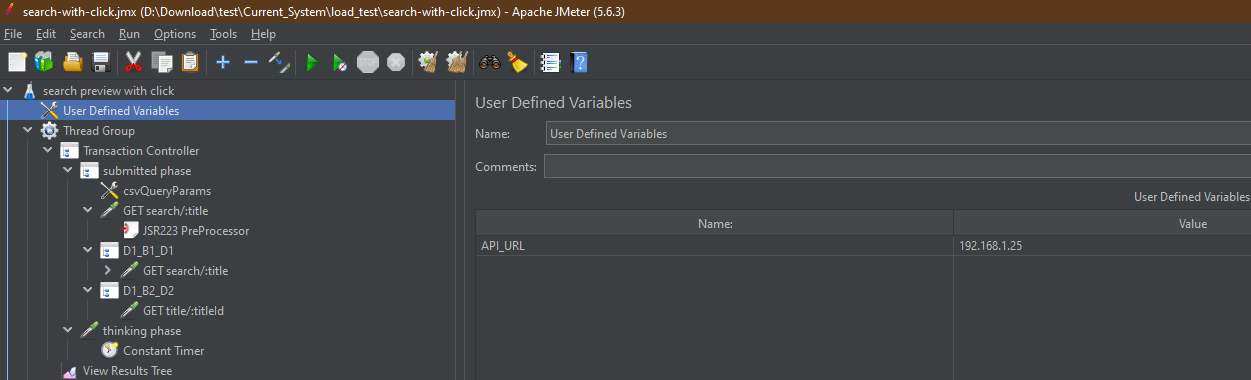
\includegraphics[width=\linewidth]{005/jmt-user-defined-variable.png}
	\caption{JMT -- User Defined Variables}
\end{figure}

\clearpage

In the ``Thread Group'' module, a population of 500 users was specified (this value will be updated automatically).
The \textit{ramp-up} period is 0, which means that when the test is initiated, all threads are simultaneously spawned in the thinking station.
The \textit{loop count} is infinite, which means that requests to the API will continue indefinitely, based on the query set imported via CSV.
The thread lifetime (\textit{duration}) is 10 minutes, after which it will eventually die.
\begin{figure}[h]
	\centering
	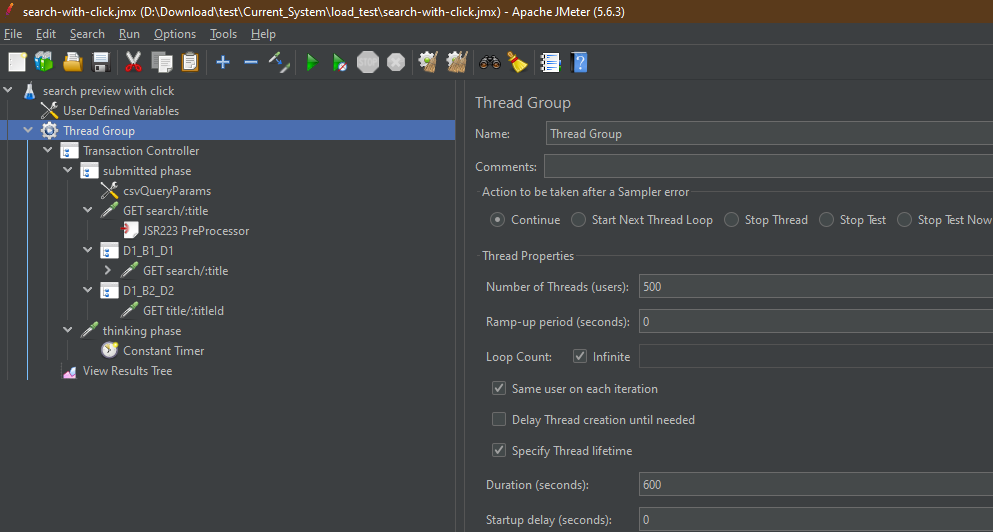
\includegraphics[width=\linewidth]{005/jmt-thread-group.png}
	\caption{JMT -- Thread Group}
\end{figure}

In the ``csvQueryParams'' module, the location of the CSV file containing the query set of 10,000 films was specified.
The file will be read cyclically by each thread and will also be shared among them, which will therefore start reading it from different rows.
\begin{figure}[h]
	\centering
	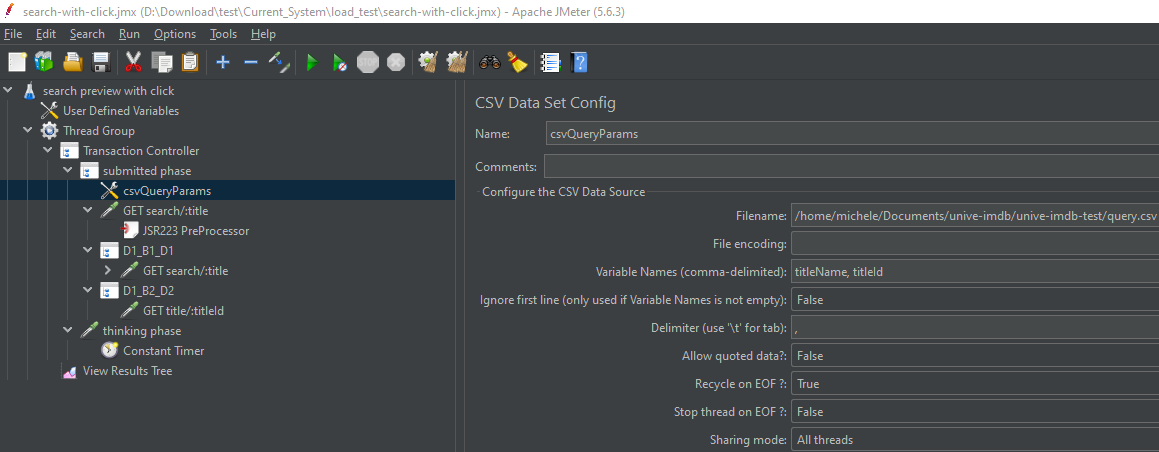
\includegraphics[width=\linewidth]{005/jmt-csv-query-params.png}
	\caption{JMT -- CSV Query Params}
\end{figure}

\clearpage

In this ``JSR223 PreProcessor'' module, the page number, which will subsequently be used to parameterize the API request ``\verb|/search/:title?page=n|'', is initialised to 1.
Additionally, a variable responsible for probabilistic routing, which will take values between 1 and 10 inclusive, is also initialised.
\begin{figure}[h]
	\centering
	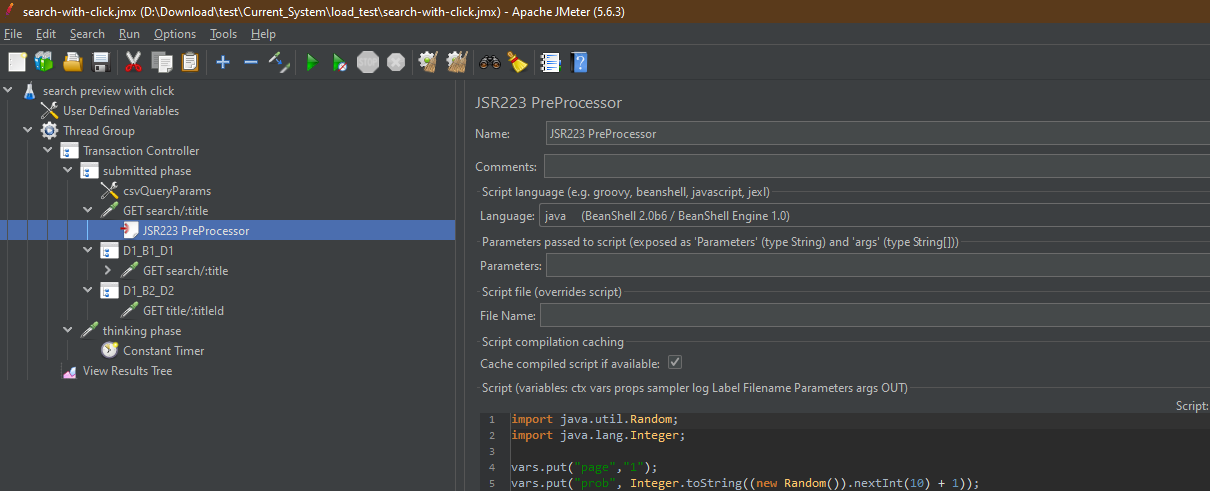
\includegraphics[width=\linewidth]{005/jmt-preproc-1.png}
	\caption{JMT -- JSR223 PreProcessor (1)}
\end{figure}

In this ``HTTP Request'' module, a request is submitted to the \newline ``\verb|/search/:title?page=1|'' endpoint.
\begin{figure}[h]
	\centering
	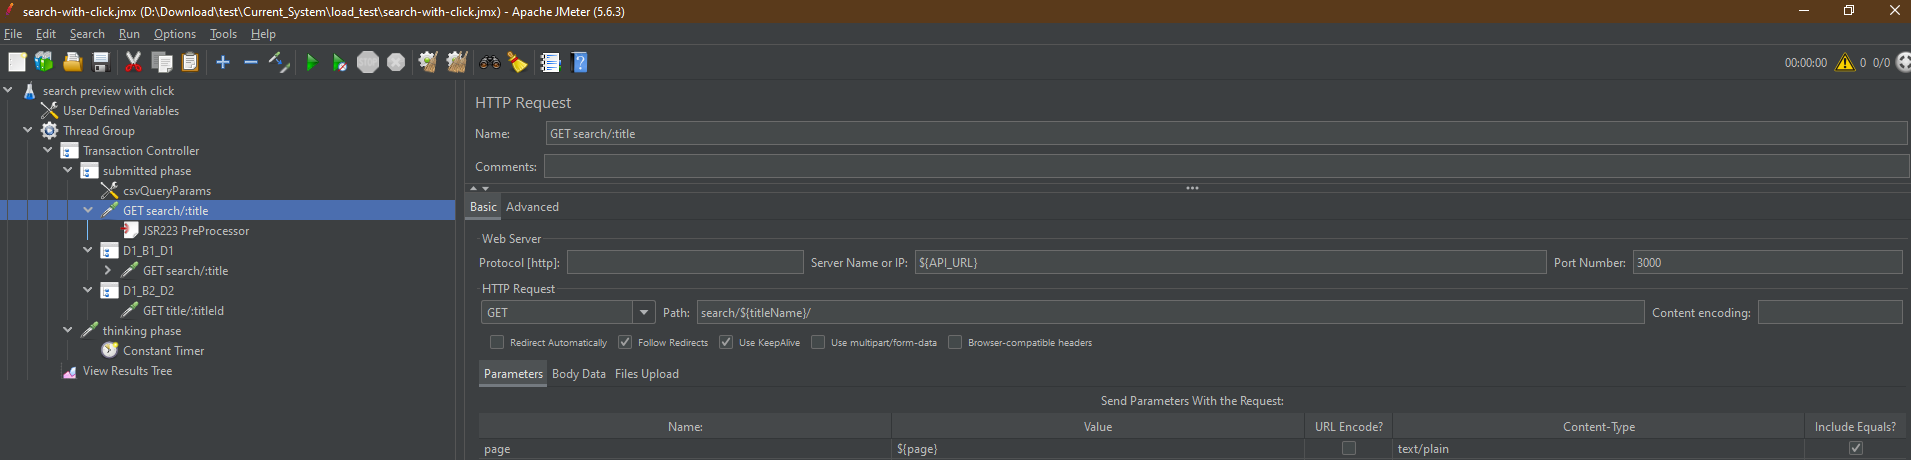
\includegraphics[width=\linewidth]{005/jmt-search-p1.png}
	\caption{JMT -- HTTP Request (1)}
\end{figure}

\clearpage

In the ``While Controller'' module, we test whether the user is within the 10\% probability of repeating the title search with an updated pagination value.
\begin{figure}[h]
	\centering
	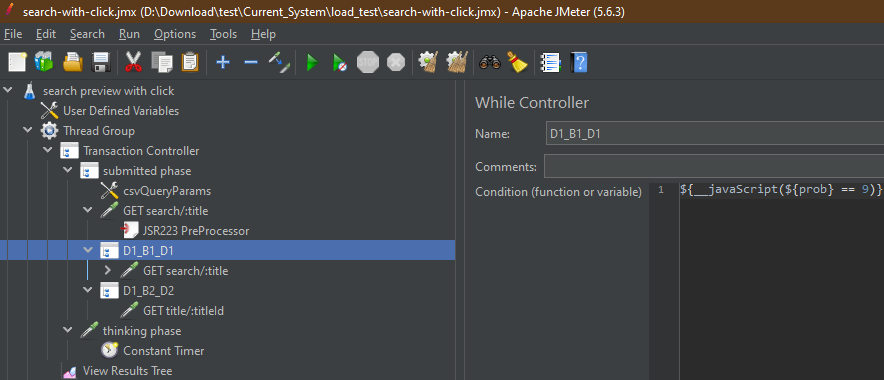
\includegraphics[width=\linewidth]{005/jmt-while.png}
	\caption{JMT -- While Controller}
\end{figure}

In this ``JSR223 PreProcessor'' module, the page number is incremented in accordance with the occurrence of the event in which the search is reiterated.
\begin{figure}[h]
	\centering
	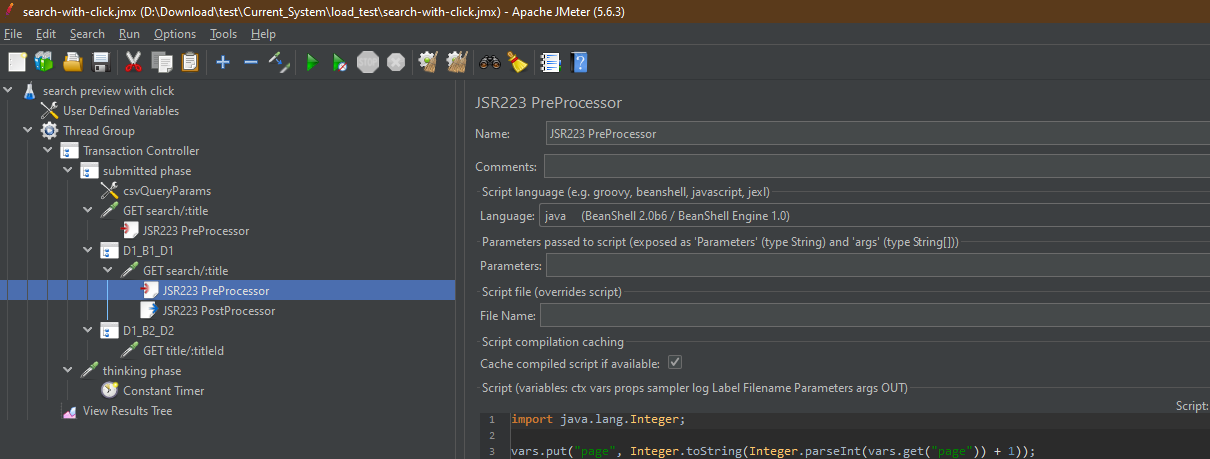
\includegraphics[width=\linewidth]{005/jmt-preproc-2.png}
	\caption{JMT -- JSR223 PreProcessor (2)}
\end{figure}

\clearpage

In this ``HTTP Request'' module, a request is submitted to the \newline ``\verb|/search/:title?page=n|'' endpoint.
\begin{figure}[h]
	\centering
	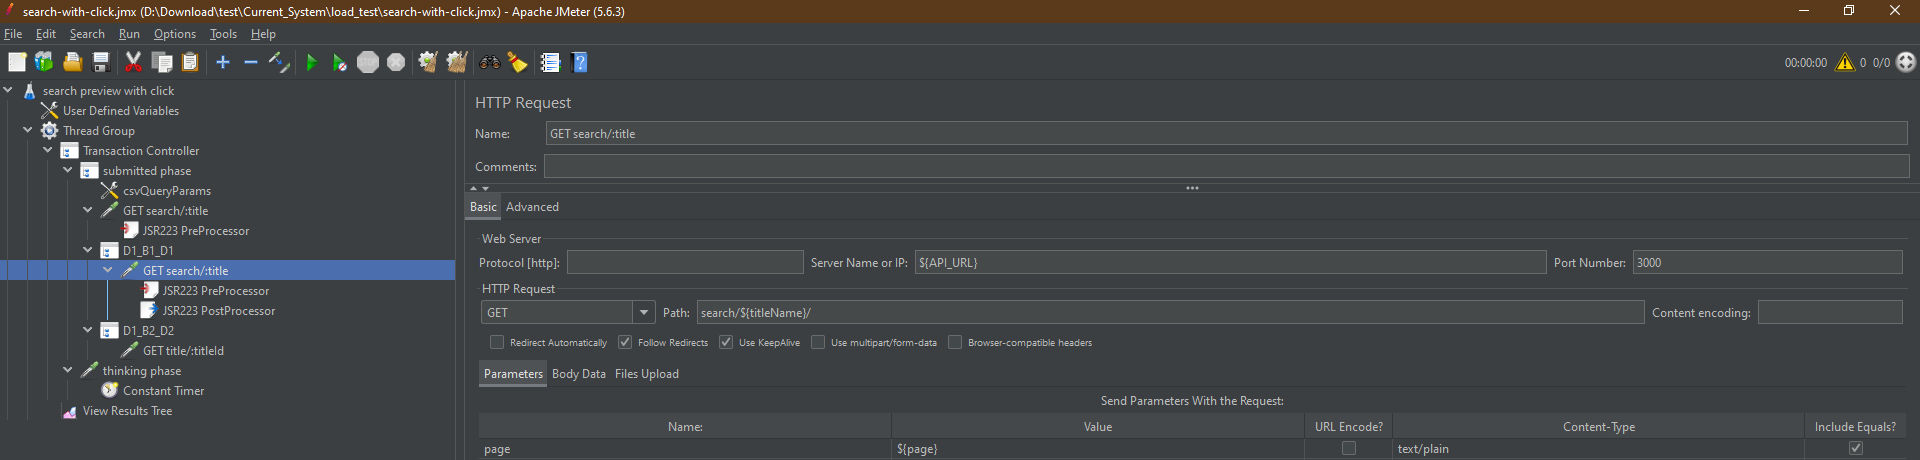
\includegraphics[width=\linewidth]{005/jmt-search-pn.png}
	\caption{JMT -- HTTP Request (2)}
\end{figure}

In the ``JSR223 PostProcessor'' module, the value is reassigned to the variable responsible for probabilistic routing.
\begin{figure}[h]
	\centering
	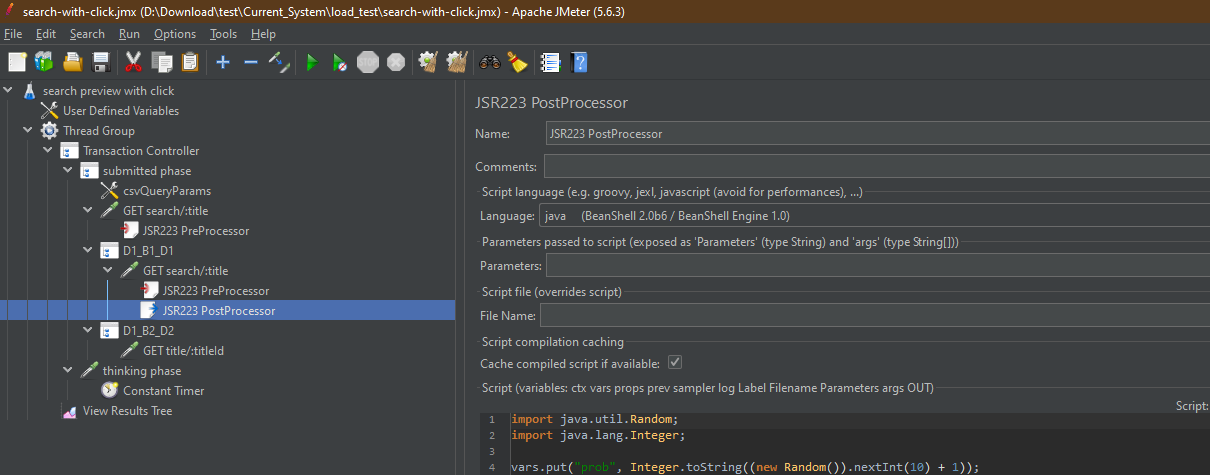
\includegraphics[width=\linewidth]{005/jmt-postproc.png}
	\caption{JMT -- JSR223 PostProcessor}
\end{figure}

\clearpage

In the ``If Controller'' module, we assess whether the user is within the 80\% probability of performing a precise search to retrieve the title or episode information.
\begin{figure}[h]
	\centering
	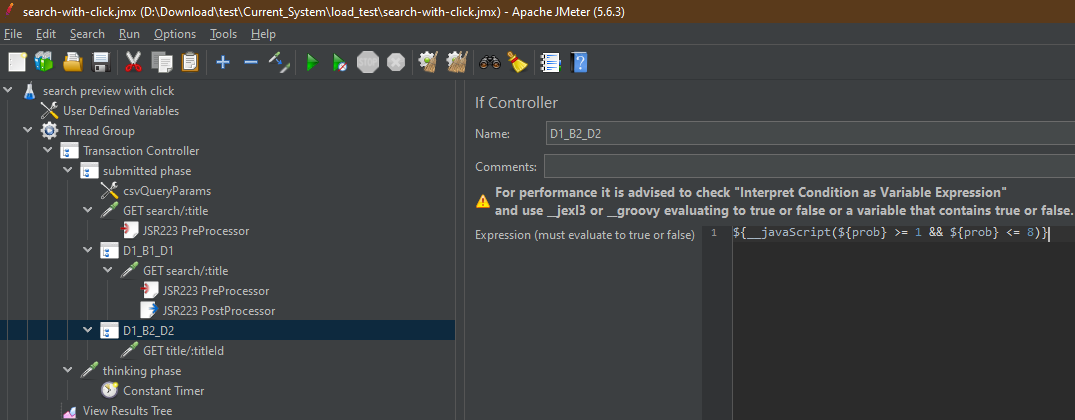
\includegraphics[width=\linewidth]{005/jmt-if.png}
	\caption{JMT -- If Controller}
\end{figure}

In this ``HTTP Request'' module, a request is submitted to the ``\verb|/title/:id| \textit{or} \verb|/episode/:id|'' endpoint.
\begin{figure}[h]
	\centering
	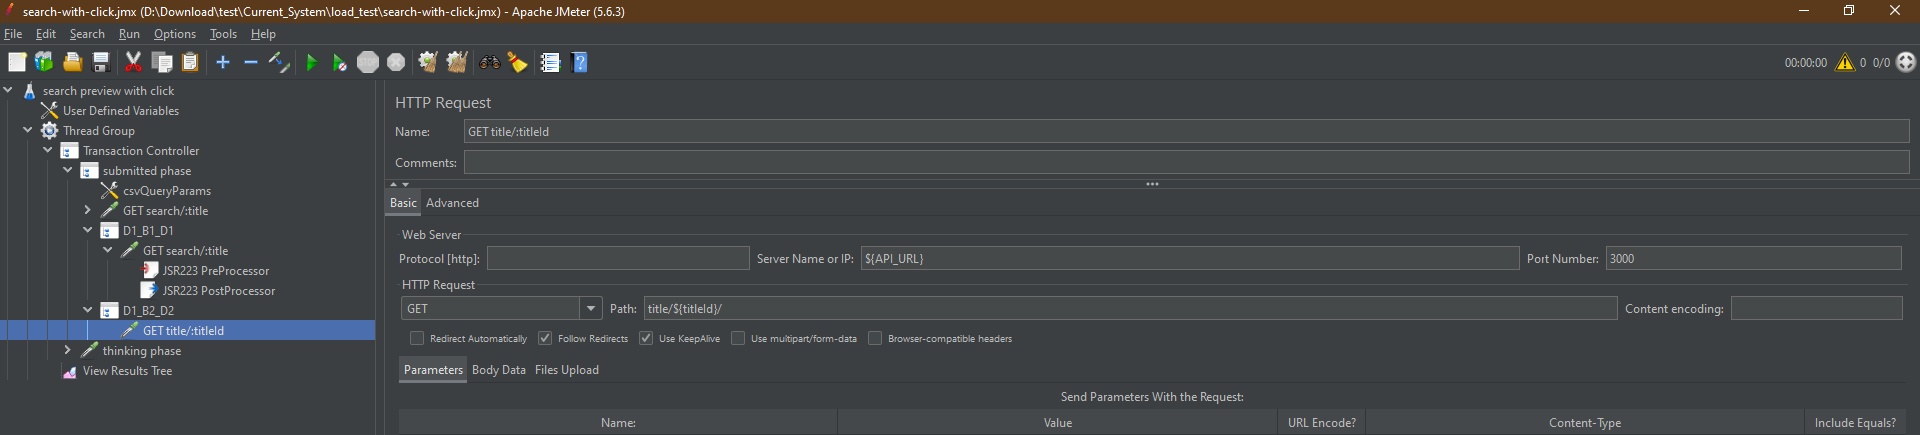
\includegraphics[width=\linewidth]{005/jmt-search-title.png}
	\caption{JMT -- HTTP Request (3)}
\end{figure}

\clearpage

In the ``Constant Timer'' module, the thinking time of 1 second is defined as the period of time that a thread will wait at the conclusion of one of its cycles before initiating a new one.
\begin{figure}[h]
	\centering
	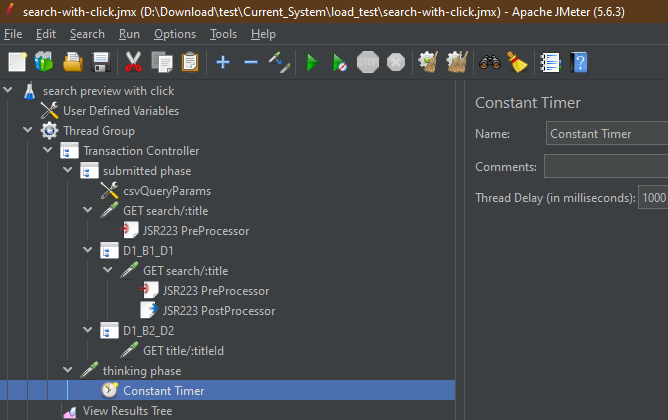
\includegraphics[width=\linewidth]{005/jmt-thinking-time.png}
	\caption{JMT -- Constant Timer}
\end{figure}

\section{Load test execution}

\subsection{Express and MongoDB configuration}

Prior to executing the load test, it is of crucial importance to ensure that the RESTful API and the database have been properly configured.

With regard to Express, it is necessary to compile and subsequently run the testing version of the script, which is relieved of profiling mechanisms and is also controlled by \verb|nodemon|\footnote[1]{https://nodemon.io/}, a Node.js npm package that among its various features automatically restarts the service when an error occurs.

With regard to MongoDB, it is essential to ensure that the Query Plan Cache is free of any residual data.
This can be achieved by executing the command \verb|db.collection.getP|\newline\verb|lanCache().clear()| within \verb|mongosh|.
Furthermore, it is necessary to disable the MongoDB Profiler by executing \verb|db.setProfilingLevel(0, { <options> })|.
Finally, if desired, the Profiler collection can be cleared with \verb|db.system.profile.drop()|.

It should be noted that the testing version of the RESTful API has been equipped with a mechanism to automatically clear the database cache after each query.
This is to prevent the distortion of test results due to caching mechanisms, which could otherwise occur if identical sequential queries were to be executed.

\subsection{Automated load test startup}

To ensure an absolute minimum of potential error in the load testing process, it was deemed appropriate to employ a Python utility for this specific purpose. 
The implemented source code is responsible for importing the load test configuration file, which was exported from JMeter in the jmx format, using the \verb|beautifulsoup|\footnote[2]{https://www.crummy.com/software/BeautifulSoup/} library.

Subsequently, the actual load test is initiated through the \verb|subprocess| library, which launches 10 sequential tests with a varying number of customers (threads), ranging from 50 to 500.

\vspace{8mm}

\begin{lstlisting}[language=Python, caption={Python script for automated load test startup}, label={lst:python-script}]
import subprocess
from tqdm import tqdm
from bs4 import BeautifulSoup

def test(name:str):
 jmx_name=f'{name}.jmx'

for n_users in tqdm(range(50, 550, 50)):      
 with open(jmx_name) as f:
  Bs_data = BeautifulSoup(f.read(), "xml")
  tag=Bs_data.find('intProp', {"name":"ThreadGroup.num_threads"})
  tag.string = str(n_users)

with open(jmx_name, 'w') as f:
 f.write(str(Bs_data))
 results_path = f'results_{n_users}'
 subprocess.Popen(f'jmeter -n -t {jmx_name} -l {results_path+"/results.csv"} -e -o {results_path}', shell=True, stdout=subprocess.DEVNULL).wait()

if __name__ == "__main__":
 test('filename')
\end{lstlisting}

\section{Load test empirical results}

The graphs of throughput and expected response time, calculated from the load test performed with JMeter, are presented below.
The graphs were generated following a parsing step of the statistics exported in JSON format from the benchmark software.

\clearpage

\begin{figure}[h]
	\centering
	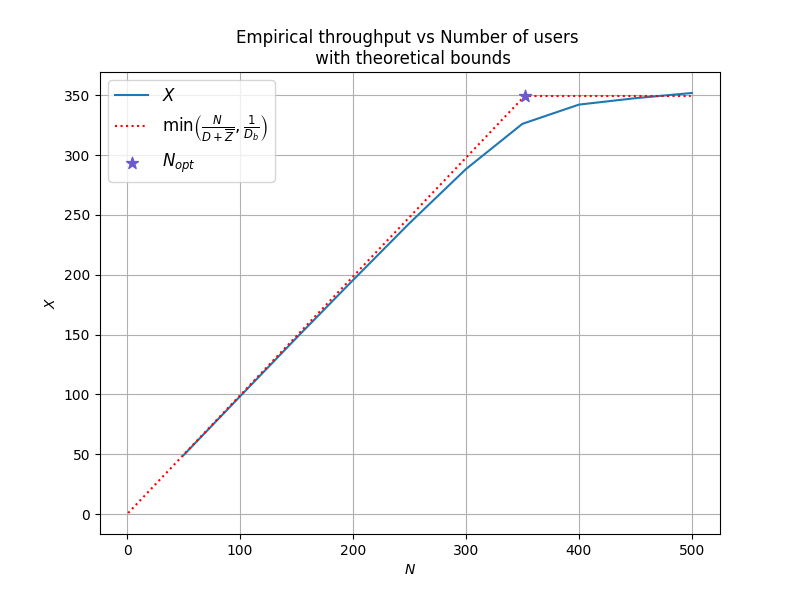
\includegraphics[width=\linewidth]{005/load-test-x.png}
	\caption{JMeter Load test -- Throughput}
\end{figure}

\clearpage

\begin{figure}[h]
	\centering
	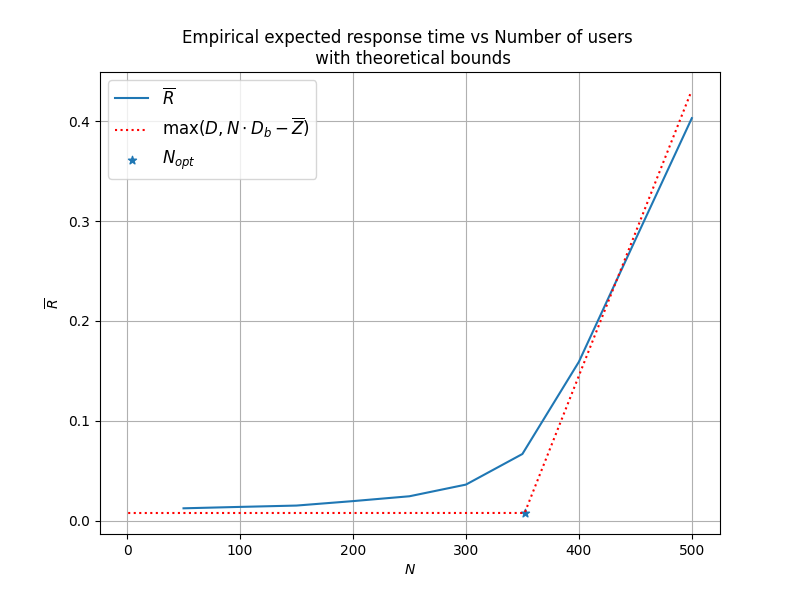
\includegraphics[width=\linewidth]{005/load-test-r.png}
	\caption{JMeter Load test -- Expected Response Time}
\end{figure}

The graphs demonstrate a satisfactory fit with respect to the analytically calculated asymptotes.
Additionally, they illustrate the precision of the estimated optimal number of users that the system can handle, which was previously determined through analysis.
